\section{The Gradient Descent Algorithm}

\vspace{-0.4cm}
To train neural networks effectively, we employ the (Stochastic) \textbf{Gradient Descent algorithm} in combination with \textbf{Backpropagation}. Backpropagation, a method for computing gradients, is crucial for updating the parameters of the neural network during training. We will delve into it shortly, but first, let's explore Gradient Descent and its significance.
\vspace{-0.4cm}

\subsection{Understanding the Gradient}

Gradient Descent is a fundamental optimization algorithm used to minimize the loss function of a neural network by iteratively adjusting its parameters. The goal is to find the optimal set of parameters that result in the lowest possible loss. The algorithm works by iteratively moving in the \textbf{direction of the steepest descent of the loss function} with respect to the parameters. This direction is determined by the \textbf{negative gradient} of the loss function, which is why we will utilize the negative sign in the algorithm.

Mathematically, the update rule for the parameters \( w \) in Gradient Descent can be expressed as:
$$
\Delta_w L = \left[ \frac{dL}{dw_1}, \frac{dL}{dw_2}, \ldots , \frac{dL}{dw_N}\right]
$$
where \( \Delta_w L \) represents the change in the loss function \( L \) with respect to the parameters \( w \), and \( \frac{dL}{dw_i} \) denotes the partial derivative of the loss function with respect to the \( i \)-th parameter \( w_i \).

Below we show a figure illustrating the partial derivatives of a function. The figure is represented in two ways: in a 3D graph and in the two-dimensional projection of the same graph (top view). The surface of the graph represents the function, where the lowest point is colored blue and the highest point is colored red. The black arrows extending from the surface indicate the direction and intensity of the gradient change of the function at each point in space. This visualization is crucial for understanding how Gradient Descent finds the fastest direction to reduce loss and update model weights during neural network training.

\begin{figure}[!htbp]
    \centering
    \includegraphics[scale=2]{tikz/chapter2 - Partial Derivatives.pdf}
    \caption{Visualization of Partial Derivatives in Two Distinct Ways}
\end{figure}

Having understood partial derivatives and the role of the gradient in the optimization process, let's now look at a visual representation of how the Gradient Descent algorithm works. In the image below, we see a three-dimensional surface representing the loss function. As before, the lowest point of the surface is colored blue and represents the minimum of the loss function. The black arrows extending from the surface indicate the \textbf{path} that Gradient Descent follows \textbf{to reach the minimum}. Each arrow represents the direction and intensity of the change in the loss function at a given point in space.

\begin{figure}[!htbp]
    \centering
    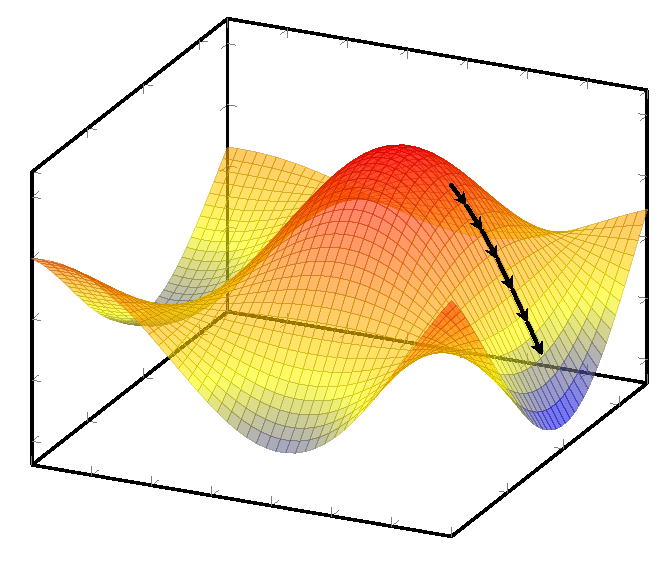
\includegraphics[scale=0.75]{tikz/chapter2 - Gradient Descent.pdf}
    \caption{Visual Representation of the Gradient Descent Algorithm}
\end{figure}

The algorithm proceeds by iteratively updating the parameters according to the gradient direction \textbf{until convergence is reached or a predefined number of iterations is completed}. By following this process, Gradient Descent effectively navigates the parameter space to find the optimal configuration that minimizes the loss function.


\subsection{The Problem of Local Minima}

In neural networks, the optimization problem is non-convex, leading to the existence of \textbf{local minima}. However, practitioners have found that these local minima are often still effective solutions. Thus, local minima are not typically a significant concern in neural network training. Below, we show an example illustrating the local minima problem for a better insight.

\begin{figure}[!htbp]
    \centering
    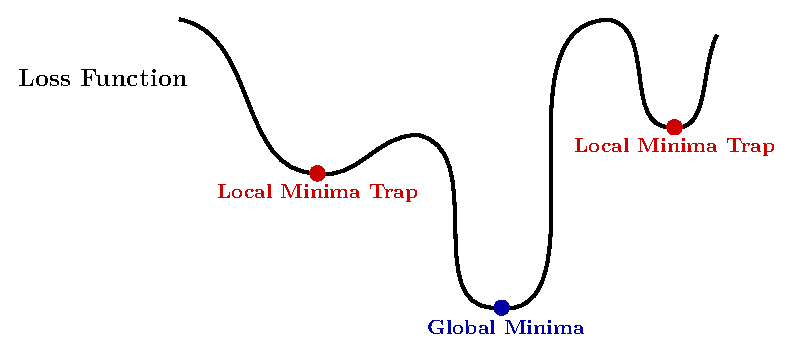
\includegraphics[scale=0.9]{tikz/chapter2 - Local Minima.pdf}
    \caption{Local and Global Minima}
\end{figure}

\subsection{The Problem of Saddle Points}

Another optimization challenge arises from saddle points, where some directions curve upwards and others downwards. At a saddle point, the \textbf{gradient is zero}, even if the point is not a minimum. Saddle points are common in high-dimensional spaces. However, they only become problematic if the optimization algorithm becomes stuck exactly at the saddle point.

\begin{figure}[!htbp]
    \centering
    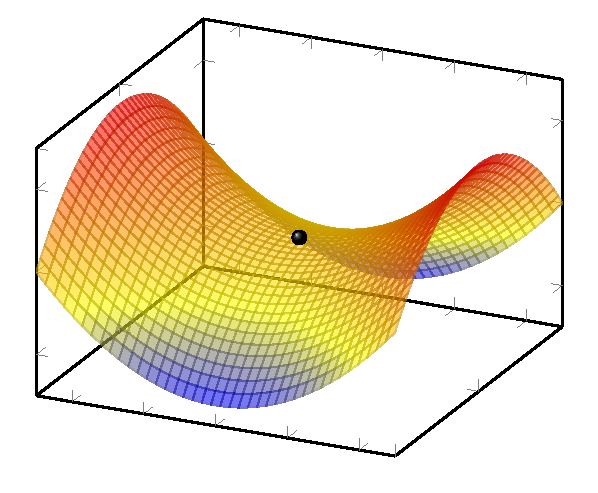
\includegraphics[scale=0.88]{tikz/chapter2 - Saddle Point.pdf}
    \caption{Saddle Point Illustration}
\end{figure}

In the figure, there is a saddle point depicted within the neural network optimization scenario, represented by the black dot. 

\section{Backpropagation Algorithm}

\subsection{Backpropagation Fundamentals}
How do we learn the weights of a neural network? Let us examine some ideas that have guided the development of learning algorithms in the context of neural networks.

The initial idea was to \textbf{randomly perturb one weight at a time}, evaluating whether that change improved model performance and saving the change. This approach, although similar to an evolutionary process, proved to be very inefficient, requiring numerous passes over the training data for each change in the weights and presenting difficulties in the last stage of learning.

Another idea involved \textbf{perturbing all the weights simultaneously} and correlating performance improvement with changes in the weights. However, this method proved equally inefficient and extremely difficult to implement.

Subsequently, a more efficient idea was proposed: to \textbf{perturb only the activations}, which are fewer in number than the weights. Although this approach is an improvement over the previous ones, it is still inefficient.

\textit{Therefore, how can we achieve more efficient learning?} This is where backpropagation comes in.

\begin{remark}
Backpropagation is a widely used learning algorithm in neural networks, which consists of three main steps:

\begin{enumerate}
    \item \textbf{Forward Propagation}: summation of inputs, production of activations and propagation of output through the network.

    \item \textbf{Error Estimation}: comparison of labels with predictions obtained from the network.

    \item \textbf{Backpropagation} of the error signal and using this signal to update the weights by computing gradients.
\end{enumerate}
\end{remark}

Starting from the training data, we do not directly know the optimal behavior of the hidden units within the neural network. However, using backpropagation, we can calculate how quickly the overall error of the network changes when we change the activity of these hidden units.

Using the derivatives of the error with respect to the hidden activities, we are able to understand \textbf{how each hidden unit affects the overall error of the network}. This allows us to gain a clear view of the separate effects that each hidden unit has on the error and how these effects are combined to determine the optimal direction to update the network weights.

Once we have calculated the derivatives of the error with respect to the hidden activities, we gain valuable information to update the weights associated with each connection in the network. This allows us to adjust the weights in a way that minimizes the overall error in the network, moving us closer and closer to the optimal solution for the learning problem.

\section{Exploring Backpropagation: Step by Step (TODO)}

Let us now describe in detail the error propagation through the neural network, starting from the output layer and proceeding to the input layer. Let's consider this neural network:

\begin{figure}[htbp]
\centering
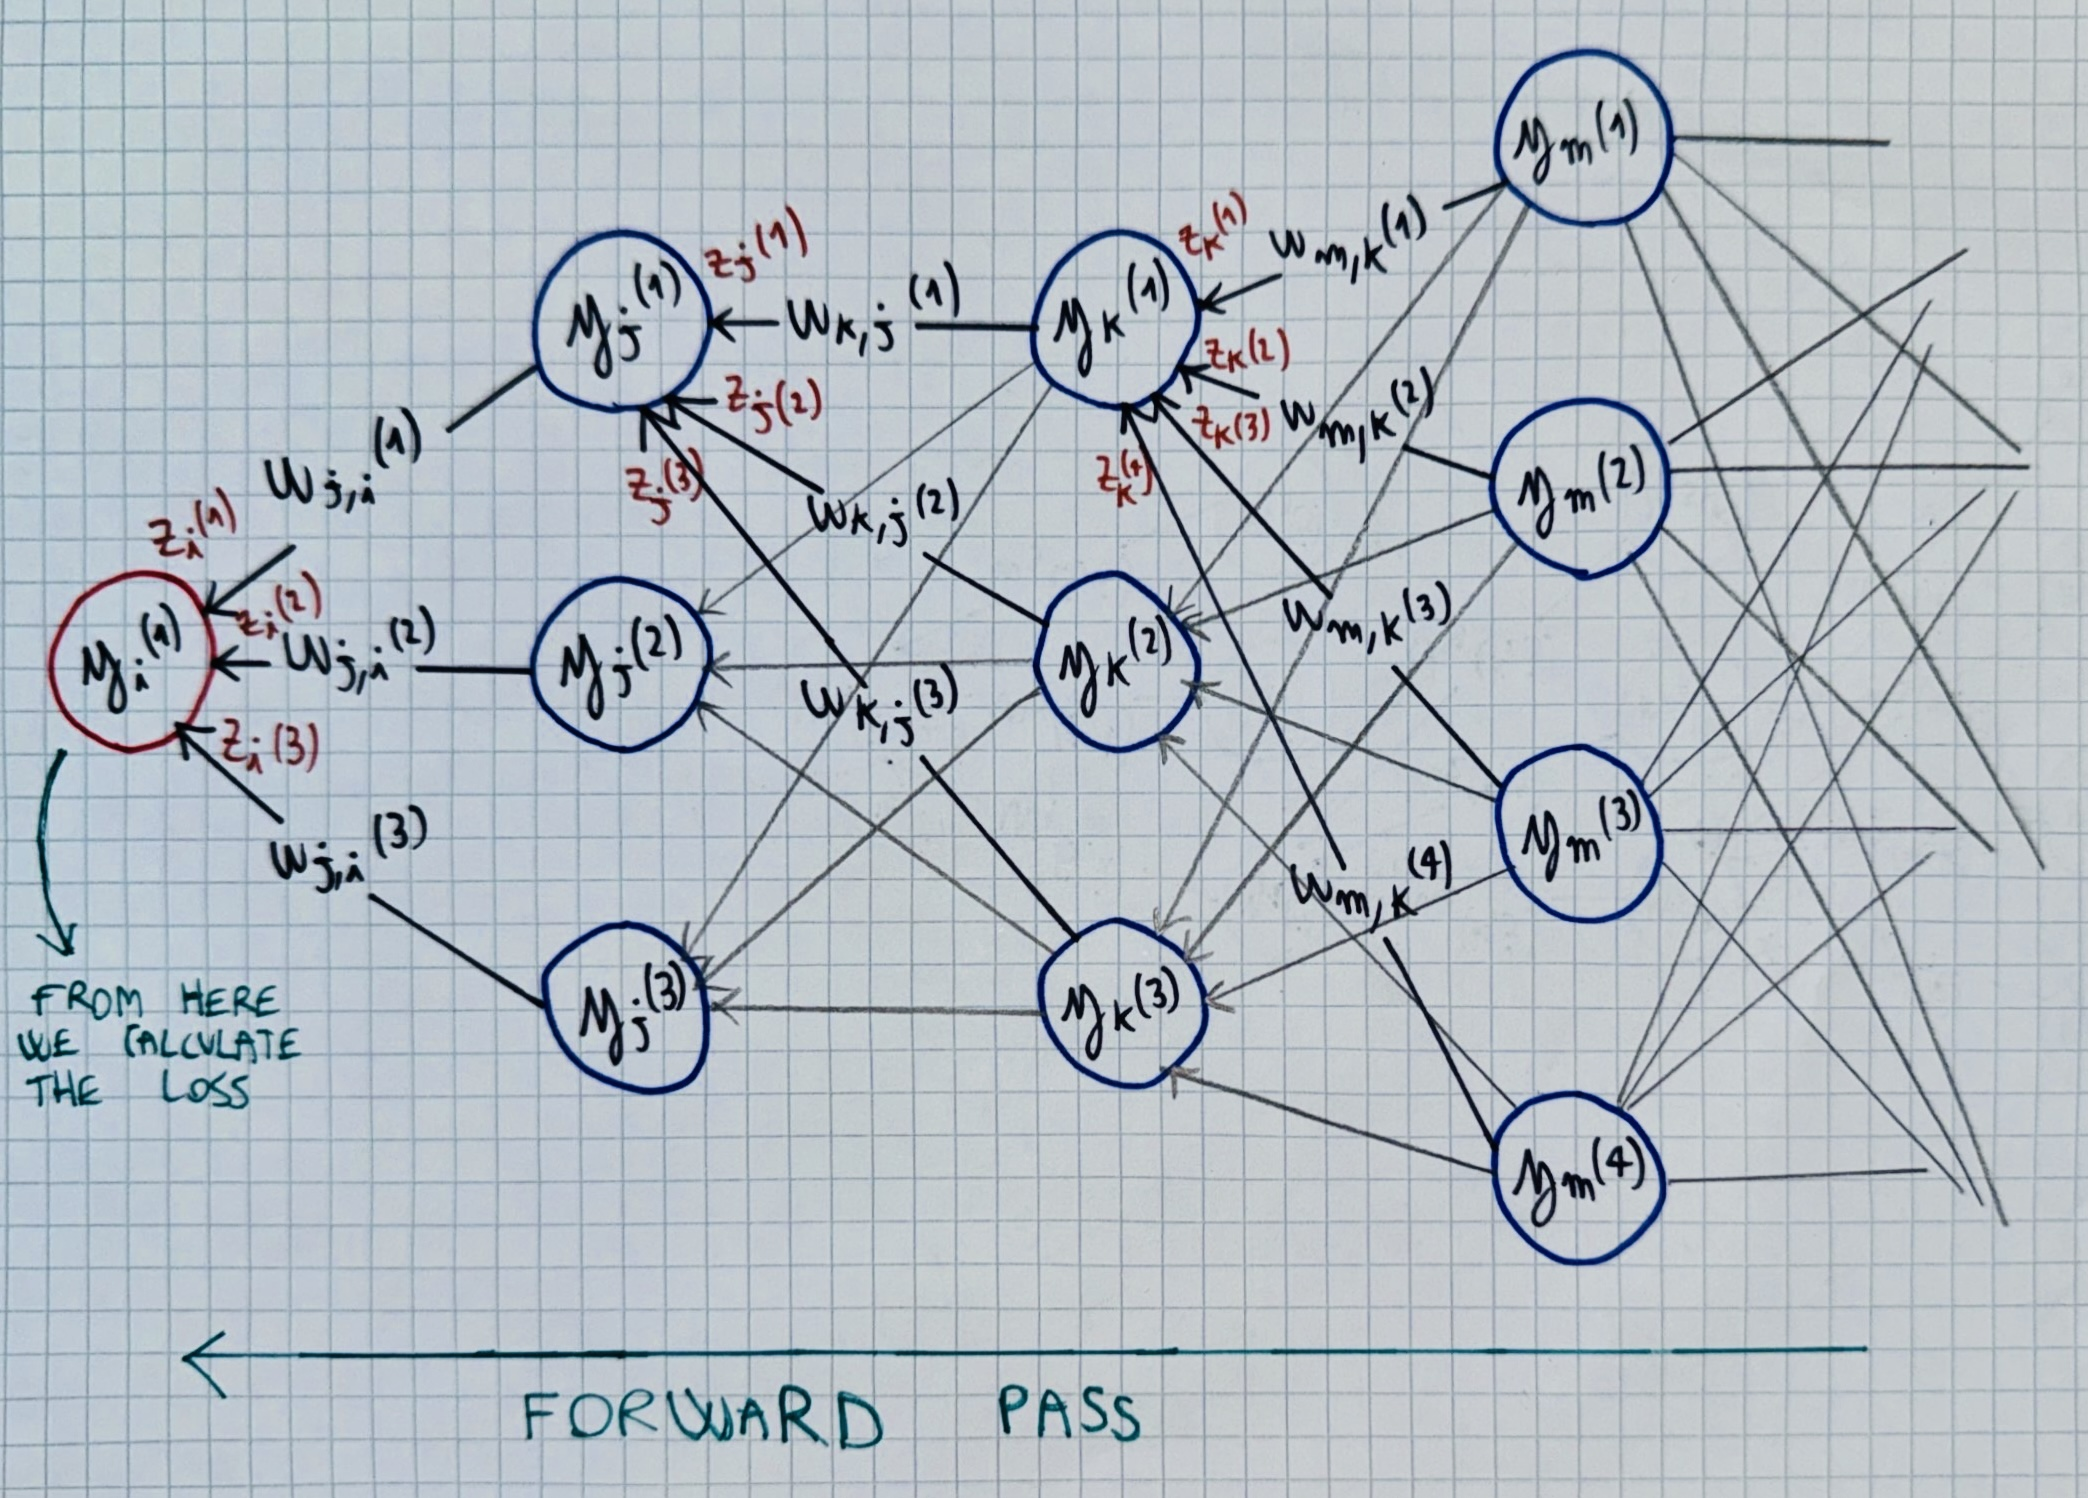
\includegraphics[width=0.8\textwidth]{tikz/chapter3 - Backpropagation.jpg}
\caption{\color{red}\colorbox{pink}{Tikz TODO}}
\end{figure}

\textbf{Output Layer}: In the output layer, after the forward pass and loss computation, we calculate the rate of change of the error with respect to the output of each node in the output layer. This is given by:
\[ \frac{d L}{d y_i} \]
Now this error is propagated backwards to the first hidden layer.

\textbf{First Hidden Layer}:
The change in the error with respect to the input (\( z_j \)) of the j-th node in the first hidden layer is given by the sum of the contributions of all nodes in the output layer multiplied by the derivative of the activation function with respect to the input of the hidden layer:
\[ \frac{d L}{d z_j} = \sum_{i=1}^{N} \left( \frac{d L}{d y_i} \cdot \frac{d y_i}{d z_j} \right) \]

Dove:
\begin{itemize}
    \item \( \frac{d L}{d y_i} \) represents the partial error with respect to the output of the output layer. (\textcolor{myred}{This was backpropagated from the output layer})
    \item \( \frac{d y_i}{d z_j} \) is the derivative of the activation function with respect to the input of the hidden layer.
\end{itemize}

\textbf{Secondo Hidden Layer}:
Once we obtain the error for the first hidden layer, we continue to propagate the error to the second hidden layer. For each node \( z_j \) in this layer, we calculate the change in the error with respect to the input (\( z_k \)) of the k-th node in the second hidden layer:
\[ \frac{d L}{d z_k} = \sum_{j=1}^{M} \left( \frac{d L}{d z_j} \cdot \frac{d z_j}{d z_k} \right) \]

Where:
\begin{itemize}
    \item \( \frac{d L}{d z_j} \) represents the change in the error from the input of the first hidden layer. (\textcolor{myred}{This was backpropagated from the first hidden layer})
    \item \( \frac{d z_j}{d z_k} \) is the derivative of the activation function with respect to the input of the next hidden layer.
\end{itemize}


\textbf{Terzo Hidden Layer}:
Proseguiamo la propagazione dell'errore al terzo hidden layer. Per ogni nodo \( z_k \) in questo strato, calcoliamo il cambiamento nell'errore rispetto all'input netto (\( z_m \)) del m-esimo nodo nel terzo hidden layer:
\[ \frac{d L}{d z_m} = \sum_{k=1}^{M} \left( \frac{d L}{d z_k} \cdot \frac{d z_k}{d z_m} \right) \]

Dove:
\begin{itemize}
    \item \( \frac{d L}{d z_k} \) rappresenta il cambiamento nell'errore rispetto all'input netto del secondo hidden layer. (\textcolor{myred}{This was backpropagated from the second hidden layer})
    \item \( \frac{d z_k}{d z_m} \) è la derivata della funzione di attivazione rispetto all'input netto dell'hidden layer successivo.
\end{itemize}

\textbf{E così via}:
Proseguiamo la propagazione dell'errore fino all'output layer in questo modo.

\textbf{Pesi}:
Infine, calcoliamo il cambiamento nell'errore rispetto ai pesi tra l'input layer e il primo hidden layer:
\[ \frac{d L}{d w_{ij}} = \frac{d L}{d z_j} \cdot \frac{d z_j}{d w_{ij}} \]

Dove:
\begin{itemize}
    \item \( \frac{d z_j}{d w_{ij}} \) rappresenta l'input \( x_i \) del nodo moltiplicato per il peso associato.
\end{itemize}

Questi passaggi costituiscono l'essenza della backpropagation attraverso una rete neurale con quattro hidden layer. Ogni strato riceve l'errore dallo strato successivo e lo propaga all'indietro attraverso la rete, consentendo il calcolo del gradiente dell'errore rispetto ai pesi e agli altri parametri della rete.
